\documentclass[preprint]{elsarticle}
\biboptions{round, numbers}
\usepackage[latin1]{inputenc}
%\usepackage[T1]{fontenc}
%\usepackage{textcomp}
\usepackage{graphicx}
\usepackage{color}
%\usepackage{setspace}
\usepackage{url}
\usepackage[english]{babel}

%Usa nombres m�s cortos y sin espacios para ficheros, dan menos problemas. Tambi�n faltaba un fichero .bst, que he a�adido. 

\begin{document}

\begin{frontmatter}

%%%%%%%%%%%%%%%%%%%%%%%%%%%%%%%   TITLE   %%%%%%%%%%%%%%%%%%%%%%%%%%%%%%%

\title{A Review on Corporate Security Solutions. A Comparison with a User-Centric and Self-Adaptive System}
% review on o review of? - JJ
%%%%%%%%%%%%%%%%%%%%%%%%%%%%%%%   AUTHORS   %%%%%%%%%%%%%%%%%%%%%%%%%%%%%%%

\author{P. de las Cuevas, A.M. Mora, J.J. Merelo}
\ead{\{paloma, amorag, jmerelo\}@geneura.ugr.es}
\address{Departamento de Arquitectura y Tecnolog�a de Computadores.\\ ETSIIT - CITIC. University of Granada, Spain}
%\author{A. M. Mora}
%\ead{amorag@geneura.ugr.es}
%\address{Departamento de Arquitectura y Tecnolog�a de Computadores. Escuela T�cnica Superior de Ingenier�as Inform�tica y de Telecomunicaci�n. CITIC. University of Granada, Spain}

%\maketitle

%
%%%%%%%%%%%%%%%%%%%%%%%%%%%%%%%%%   ABSTRACT   %%%%%%%%%%%%%%%%%%%%%%%%%%%%%%%%%
%
\begin{abstract} 
Enterprises, and particularly their Chief Security Officers (CSOs), want to make sure that their Security Policies are complied. % fulfilled? Met? - JJ
 This goal has become hard to achieve since employees are able to use their own devices (laptops, smartphones, and tablets) at work, or at home but for work purposes. Since this is part of the Bring Your Own Device (BYOD) philosophy and is being adopted by many companies every day, a number of solutions have arisen in order to adapt it securely. In this paper, the most relevant solutions are presented, describing their main features. In addition a novel system being developed inside the European Project MUSES (Multiplatform Usable Endpoint Security), is also introduced and compared with these existing solution. % No puedes comparar soluciones existentes con soluciones propuestas hasta que no haya un prototipo. Debes dejar claro esto o te lo van a echar en cara - JJ
 This system is able to cope with security issues regarding the enterprise security policies, but is a user-centric tool, which considers system user's behaviour in order to adapt or even increase the defined set of security rules. MUSES applies machine learning and computational intelligence techniques in order to do this, and also is able to predict future security incidences produced by these users. % �applies en presente o will apply en el futuro? Si haces "claims" tienes que probarlos - JJ
\end{abstract}

%
%%%%%%%%%%%%%%%%%%%%%%%%%%%%%%%%%   KEYWORDS   %%%%%%%%%%%%%%%%%%%%%%%%%%%%%%%%%
%
\begin{keyword}
Corporate mobile security \sep End-to-end security solutions \sep User-centric systems \sep Self-adaptation \sep Multiplatform \sep Information Asset \sep Security Policies \sep Data security and data privacy \sep BYOD.
\end{keyword}

\end{frontmatter}


%-------------------------------------------------------------------------------
%%%%%%%%%%%%%%%%%%%%%%%%%%%%%%%   INTRODUCTION   %%%%%%%%%%%%%%%%%%%%%%%%%%%%%%%
%-------------------------------------------------------------------------------

\section{Introduction}
\label{sec:intro}

The way how data has been stored and accessed in the companies has
completely changed over the last few years. %Pru�balo. Debes tratar de
                                %probar todas las afirmaciones que
                                %incluyas - JJ 
 The use of company-owned servers being accessed from desktop PCs (and
 maybe laptops) from within the company facilities has been
 transformed into the distribution of these data among a number of
 machines, even not all belonging to the company, and % este and es de
                                % "the distribution", as� que no
                                % puedes usar un gerundio - JJ
working over the famous Cloud Computing environment. Besides, being
stored in the cloud or not, data are %data es colectivo, por tanto
                                %singular, aunque tambi�n se puede
                                %usar are
                                %http://www.theguardian.com/news/datablog/2010/jul/16/data-plural-singular
                                %- JJ
 being consulted and modified through a wide amount of devices, some
 of them owned by the company's users. This is the so-called Bring
 Your Own Device (BYOD) philosophy. It is becoming highly successful
 due to the impact that portable devices (such as smartphones and
 tablets) are having in the market. % no references so far: bad - JJ
Data security and privacy are key factors for a company, thus, to
protect them, it is usual to define Organisational Security
Policies. Their definition is nowadays a very difficult problem, since
the BYOD tendency %No lo has definido - JJ
 means that several factors must be considered \cite{Opp_Security11}, most of them previously ignored or non considered in security systems, for instance the current mixture between personal and professional information in these devices (the user could navigate inside social networks where there could be friends and also company partners or clients).

In this scenario several solutions have arisen in order to manage the
corporate security. Some of them are focused only on smartphones, while others are thought for laptops; also some are implemented for a certain platform, but others consider multiplatform. However most of them try to be non-intrusive (regarding the users' personal data), friendly and easy to use. 
This paper presents an overview of the main solutions, describing their features, advantages and flaws. 

Moreover, % moreover qu�? La �ltima frase se refiere a lo que hace
          % este trabajo - JJ
it has been demonstrated that people are the main hazard regarding the company security \cite{Adams_Users05}, so in this situation, some monitorization and security-aimed applications are arising, aiming to cope with the concept of seamless working experience on different devices. 
This concept is a methodology of work which allows users to start/continue a working session over multiple devices and locations without any significant loss of data. This new situation has a big impact from the point of view of the security \cite{Schu_SecPatterns05}, since the company's data borders have changed in the last years so now the users can access significant data from outside the enterprise, and possibly through a non absolutely secure channel.

Thus, this work also introduces a novel (still in development) system
named MUSES, from Multiplatform Usable Endpoint Security, which is a
device-independent end-to end user-centric tool, based in a set of
security rules defined as specifications of the Company Security
Policies, but with the capability of `learning' from the user's past
behaviour and adapt, even inferring new ones, the set of rules in
order to deal with potential future security incidents due to the
user's. Then will react, in a non-intrusive way, to the potentially
dangerous sequence of actions (events) that he or she is conducting at
any time. % lo de he or she deber�as quit�rtelo de enmedio. O usas he
          % o she, aclarando al principio lo que quieres hacer - JJ

To this end MUSES will analyse the users' behaviour by means of Data
Mining (DM) techniques \cite{DataMining_Lee01} and Machine Learning
(ML) methods \cite{MachineLearning_Bishop06}, extracting a set of
patterns which will be later processed by means of Computational
Intelligence (CI) algorithms \cite{}. % trabajo futuro no debe estar
                                % en la intro. Lo que quieras o no
                                % quieras hacer no prueba nada - JJ

MUSES will include some important modules in the loop, such as an
Event Processor, which performs an event correlation task
\cite{SurveyEventCorrelation_Tiffany02}, matching occurred events with
rules to deal with them and extracting threads that a Real-Time Risk
and Trust Analysis Engine (RT2AE) \cite{RT2AE_SOTICS13} will process
(along with other trust data and profiles), to select the best
subset. % �Es un overview o un "position paper"? Si vas a hablar de
        % muses tambi�n debes decirlo en el t�tulo.  JJ

In the paper a comparison between the rest of solutions and MUSES is
also conducted, focusing on the advances beyond the state of the art
that this novel system (being developed inside an European Project of
the same name) will bring.  % en esta comparaci�n Muses falla una
                            % caracter�stica b�sica: "existencia". Yo
                            % lo incluir�a como trabajo futuro
                            % solamente en vez de hacer tanto
                            % �nfasis. 

The rest of the paper is organized as follows. First, some background
situation about enterprise security is presented in Section
\ref{sec:preliminaryconcepts}, explaining how BYOD philosophy affects
it. % "it" ser�a "background" en este caso. Si no te refieres a �l
    % simplemente pon el sustantivo entero - JJ
Then, some solutions from different companies are detailed in Section
\ref{sec:toolsreview}, even if they are still in development.   % no
                                % cualifiques esto. "Present and near
                                % future", por ejemplo. 
Then, in Section \ref{sec:muses}, the Multiplatform Endpoint Security
System is presented. Its advantages and benefits in comparison with
the other solutions are commented in Section
\ref{sec:comparison}. %Siendo que muses no existe, yo no le dedicar�a
                      %una secci�n aparte - JJ
Finally, the conclusions are discussed in Section \ref{sec:conclusions}.


%----------------------------------------------------------------------------
%%%%%%%%%%%%%%%%%%%%%%%%%%%%%%%   BACKGROUND  %%%%%%%%%%%%%%%%%%%%%%%%%%%%%%%
%----------------------------------------------------------------------------


\section{Preliminary concepts and background about enterprise security}
\label{sec:preliminaryconcepts}

Until these days, %cu�les d�as? - JJ
 enterprises used to follow a static Security Policy devoted to controlling a certain structure \cite{BYOD13}, where the Information Assets and the devices were purchased and maintained by the company. Now that corporate networks are becoming dynamic for being adapted to the BYOD philosophy, there is an additional risk because the devices that the employees use are not always company-owned. A needed security policy, or in this case, an Information Security Policy (ISP from now on) should deal with the way of protecting a certain organization's information against a security breach. Though there are standards, such as the ISO27002 or the Security Forum's Standard of Good Practice\footnote{https://www.securityforum.org}, and many guidelines \cite{SecPol09}; an ISP is built depending on the characteristics of the community/organisation that they are built for.

On the other hand, employee-owned devices like smartphones, are not just for work purposes anymore. As the name says, smartphones are more than simple old cellular phones, and people who use them in their works have the possibility of maintaining a good balance between work and private life. For this reason, the risk of uncontrolled devices accessing to corporate access in unsafe conditions, due to the number of risky applications is bigger.

Normally, the enterprise network architecture was being adapted to cope with external attackers \cite{MIT05}. With the incorporation of BYOD, the threat is about corporate assets being compromised due to employees' devices with vulnerabilities \cite{android11}, or leaked because they are being accessed from a device connected through an unsecure (public) network.

Thus now, more things should be considered than the usual ones when designing a company's network architecture. In Figure \ref{fig:proposed_diagram} there is a proposal which can be used for the beginning of the study of solutions that may secure such a dynamic environment. It includes the possibility of having employee-owned mobile (smartphones and tablets) and portable (laptops) devices, and also the opportunity that the employees have of connecting these devices either from inside or outside the company premises. Moreover, company's information assets are constantly accessed under these conditions, considering that an information asset means every \textit{piece of information} that has a \textit{value} (cost depending on the risk of being lost or leaked) for the company. It can be referred to files with sensitive information to certain mails, or even to company applications.

\begin{figure}[ht]
	\begin{center}
		\includegraphics[scale=0.4]{img/proposed_diagram.eps}
		\caption{Architecture approach of an Enterprise Network assuming that the Company has adopted the BYOD philosophy.}
	\label{fig:proposed_diagram}
	\end{center}
\end{figure}

The other issue to cope with is the elaboration of a good ISP, understandable for every user of the company, and more importantly, non-intrusive for him. A lot of researchers have studied the natural tendency of employees to comply with the ISP \cite{SecPolComp07,SecPolComp10,SecPolComp12}, reaching conclusions such as the employees compliance with the security policies increases educating/training them in information security awareness  \cite{SecPolComp09}, and decreases applying too much sanctions when a misuse or abuse occurs \cite{SecPolPenalty09}. Thus, in this paper, for each tool in Section \ref{sec:toolsreview} it is specified if the developers have taken into account the construction of ISPs, or even if they give some guidelines for building them.

This situation leads to a need of protecting the organisation's side, but also the users' side, making non-interfering easy-to-follow ISPs, and leaving them to use their devices for personal purposes while working, without putting organisation's information assets under risk. The compliance of these requirements would compose an End-to-End Security Solution (protecting both enterprise and employee), which is the motivation of the commented tools and, as presented in Section \ref{sec:muses}, is the aim of the MUSES project.


%------------------------------------------------------------------------------
%%%%%%%%%%%%%%%%%%%%%%%%%%%%%%%   TOOLS REVIEW  %%%%%%%%%%%%%%%%%%%%%%%%%%%%%%%
%------------------------------------------------------------------------------

\section{Tools for corporate mobile security}
\label{sec:toolsreview}

Now that BYOD philosophy is becoming a tendency, a number of tools appeared by now, and others are under development but expected to be released soon. They were specifically designed for Chief Security Officers (CSOs) and Chief Information Security Officers (CISOs) to secure, monitor, and act over spartphones and other personal mobile or portable devices, when they become too risky. Some of those tools have influenced the development of the MUSES system  itself (Section \ref{sec:muses}). The present section introduces the mentioned products, as they can be considered related to the MUSES objectives.

% Don't completely like the intro for being too focused to MUSES.
% Aparte, ya hay alg�n trabajo e informes publicados por Muses, igual
% ser�a conveniente citarlos - JJ
%----------------------------------------------------------------------------

\subsection{IBM Hosted Mobile Device Security Management}
\label{subsec:ibm}

One of the first companies who supported the BYOD model was IBM in 2011 \cite{IBM_tool}, as they recognized the increase of employees who brought their personal smartphones or tablets into the workplace. To help organizations \cite{ibm11} embracing both company and employee owned mobile devices (as said, this practise is part of the BYOD model) in a security-rich environment, IBM developed a mobile device security management solution. For IBM, a mobile security strategy should focus on several key areas.

Thus, the organization should identify which business data the strategy will allow to be stored and processed on which mobile devices. This helps to determine what needs to be protected and to what degree. Then, since different mobile platforms have different native security mechanisms, the organization needs to define which mobile device platforms will be allowed in the business environment and, thus, which need to be supported in the mobile security strategy and plan. That means, to define the scope of the security plan. Also it is needed to decide the responsibility for mobile security management work, whether using the current IT security team to handle mobile devices, or outsourcing them to a managed security service provider. And no matter what the mobile environments are, a number of mobile ISPs and best-practise procedures need to be put in place and should also be identified in the company's mobile security strategic plan.

Taking into account these considerations, IBM developed a framework that specifies security domains and levels for applying various security technologies. When applied to mobile devices (not portable ones, so that laptops are not considered), the features of this framework depend on the deployment:

\begin{description}
	\item[Identity and access] Not only the use of strong passwords when accessing the devices, but also supply two way authentication and VPN access control, by supervising the authorised IP addresses and adding re-authentication for accessing resources (assets) with high value.
	\item[Data protection] Data security stored in the devices, related to professional life, is encrypted, also during the transmission. Moreover, when a device is lost, data can be removed remotely, and the device located or locked out (locking out a device is also made after a modifiable timeout). Finally, back ups are performed periodically once the device has been recovered.
	\item[Application security] This is related to the requirement of being connected from a controlled location for authorising the download of business applications, and those applications must be certified (also the currently running on the device). Actually, IBM's tool can monitor and remove applications which are identified as untrustworthy or unsafe.
	\item[Fundamental integrity control] Running both anti-malware software and personal firewall, and making the result of these tests as dependency for VPN's intranet access. 
	\item[Governance and compliance] Taking into consideration the mobile security as an important point in the overall risk management program of the company, and extend the periodic security audits to mobile devices too.
\end{description}

The considered architecture for this solution is a client-server architecture, where the controlling center is placed in the server, and the client would be installed on the mobile devices. This way, the client/device would communicate with the server as regularly as possible, to enforce policies, execute commands, and report status. With these features, and by analysing in the server the incoming data from the devices, this IBM's solution would be able to help enterprises to support ISPs compliance and to recognise (consequently acting over) mobile threat landscapes.

%Regarding IBM hosted mobile device security solution's architecture, the solution is built on a sound client-server architecture in which the server centrally controls and manages security policies and settings for various security features. The client would be installed on the mobile device and regularly communicate with the server to enforce policies, execute commands and report status. Also, IBM's solution contains reporting and analysis capabilities, with information that helps the company to support ISP compliance, recognize the mobile threat landscape and evaluate the solution's effectiveness in countering threats.

%----------------------------------------------------------------------------

\subsection{Sophos Mobile Control}
\label{subsec:sophos}

Sophos is a company founded in 1985 focused on IT security and data protection for businesses. Their \textit{Mobile Device Management} main product \cite{Sophos_tool} is Sophos Mobile Control. It is oriented to IT administration for mobile devices, trying to offer to the users the possibility of choosing the delivery model to suit their needs, i.e., between on-premise and Software as a Service (SaaS).

The tool offers the possibility of managing all workers and co-workers smartphones and tablets from a single-based console. The console monitors the devices throughout their full life cycle: from the initial set up and enrolment, right through to decommissioning. Other features are similar to IBM's product, adding some new like being able to connect to an existing user directory using Lightweight Directory Access Control (LDAP)\footnote{LDAP is an application protocol for accessing and maintaining distributed directory information services over an Internet Protocol (IP) network.}.
	
Additional security is provided by the incorporation of \textit{Malware and Web protection}, so that the user does not need to install anti-malware software by him or herself. Regarding the compliance enforcement, the main goal is not to sacrifice company's security in favour of flexibility for the users, which has been demonstrated \cite{SecPolPenalty09} that could result in bad (unwilling or not) users' behaviour. Thus, company's BYOD initiative should include an acceptable use policy to ensure the users are aware of any measures the company may take if a device breaches any ISPs. Sophos aims to reach this by doing three main tasks: First, by enforcing IPSs, i.e. allowing setting up user and group-based security policies separately. The security settings can also vary from one platform to another, thus looking to support all of them is necessary to set task bundles and individual actions for many different violations. Secondly, by a risk mitigation in which the actions to perform can be set according to the severity of a breach. For minor cases, the company may want to simply inform to the user, but if sensitive data is at risk, a remote wipe may be the chosen option. As previously stated, the actions vary for each platform, but the most common platforms such as Android and iOS allow blocking email access, notifying the admin, performing a remote lock or wiping, locating a device using 3D maps, triggering a remote alarm, transferring a task bundle combining a number of actions, and Sophos's solution adds the possibility of trigger a scan. Finally, compliance check, i.e. though some of the most widely used features include allow or disallow root rights or jailbreaking, require encryption, and whitelist or blacklist apps. Sophos also allows disabling malware apps, setting maximum intervals since last \textit{Mobile Security scan}, and allowing or disallowing suspicious apps and potentially unwanted apps (named PUAs).
	
Then, the Enterprise App Store included in Sophos Mobile Control allows the company to supply the users with recommended and/or required apps directly on their devices. Both company's in-house and app store apps are suggested directly on the user's mobile device, so they can click to trigger the installation. Also, for keeping the employees working without increasing the burden for the IT department, the self-service portal built-in included in Sophos's solution has many features. Among others, it shall be mentioned that, wanting the employees to use their personal devices at work, they can register them (with a provided step-by-step process) and agree to an acceptable company-defined use policy. All profiles, including email access, would be available after registration, and the portal may be accessed from any PC with Internet access, or even from a mobile device itself. Furthermore, when a device is eventually stolen, users can choose to remotely locate, lock or wipe their devices and reset their passcode without having to contact the company help desk. From the company side, they can define which features are available in a self-service portal from the administrator console.

%----------------------------------------------------------------------------

\subsection{Samsung's Knox Mobile Security Suite}
\label{subsec:samsungknox}

As part of its SAFE (Samsung for enterprise) brand, Samsung revealed at the Barcelona Mobile World Congress 2013 the Knox application \cite{Samsung_tool}, which was expected to be available on its last Galaxy smartphone generation. The solution is available since December 2013.
The main feature of this security package is the use of different containers, or environments, for business and personal sides. Each one even includes its own graphic configuration (wallpapers, colours, and so on), in order to be more easily recognised and distinguished by the user.
There will be needed introducing a password to enter into the business side and, once \textit{logged in} this container, no more passwords will be required for the business applications. The applications approved by the company IT department must meet Samsung's security standards and allow single sign-on. A Knox API will also be provided for the company to be capable of accessing over almost 205 predefined IT policies (the SAFE API grows this number to 475). Also, Knox would allow different VPNs for individual apps.
Regarding the information protection methods, data files saved by applications of each environment are encrypted with AES 256-bit algorithm, in such manner that only the appropriate container can access these files. In the same way, the user won't be able to share data between the two environments, e.g. creating separate contact lists so the user cannot send a contact from one side to the other, or if the user copies data to the clipboard in the Knox container, it won't be there in the personal container. Figure \ref{fig:img_knox_01} shows the device architecture with three main parts, each one in charge of deploying some of the mentioned characteristics.

\begin{figure}[ht]
	\begin{center}
		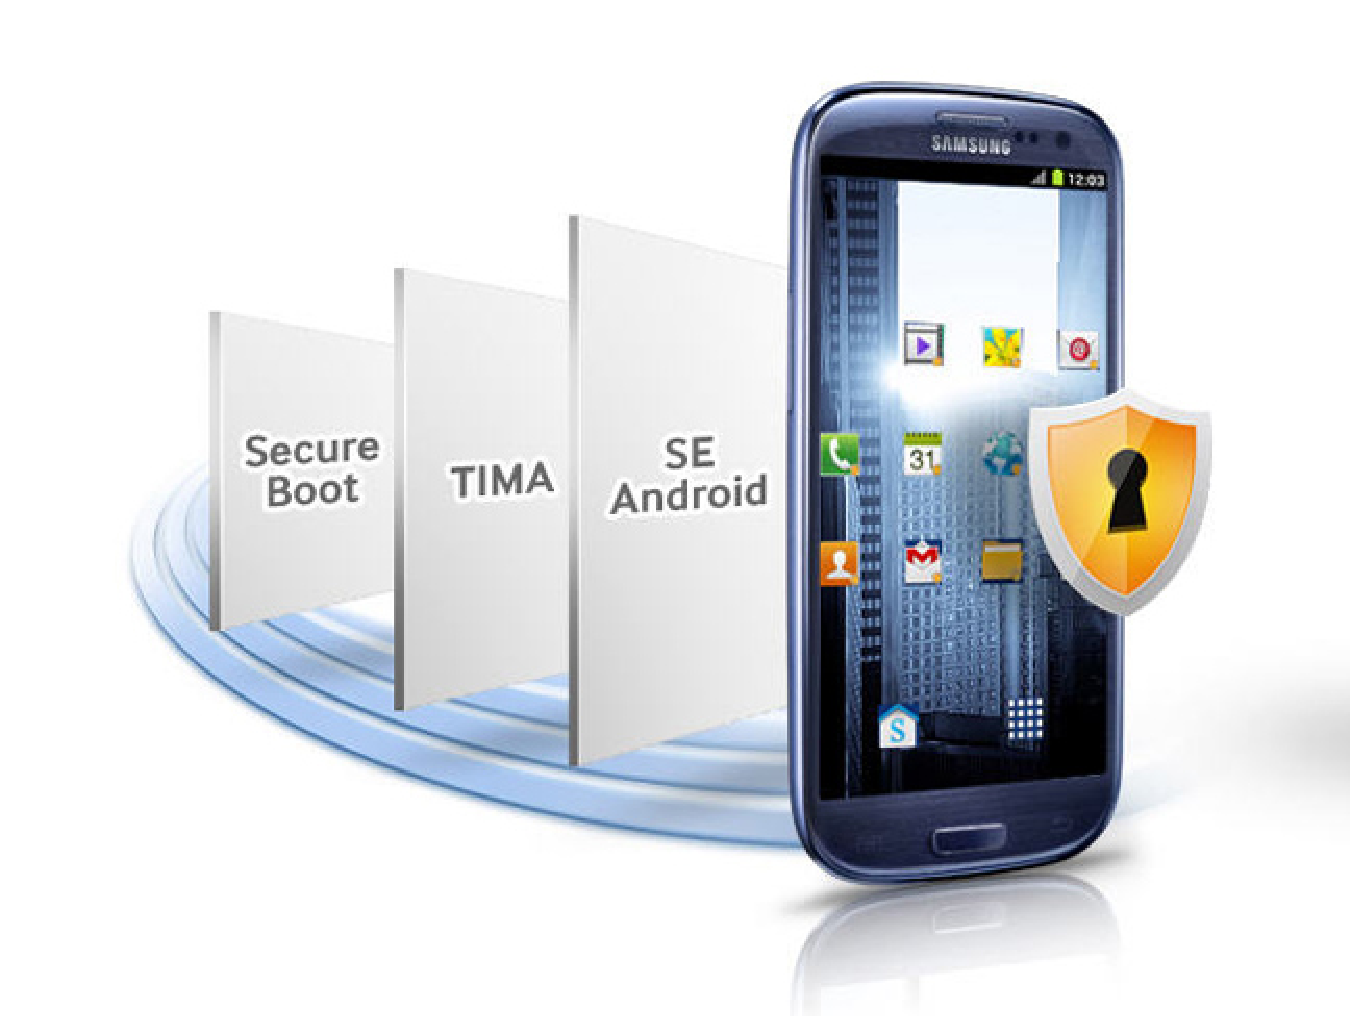
\includegraphics[scale=0.3]{img/samsung_knox_nueva.eps}
		\caption{Samsung's Knox utility architecture. Source: http://www.samsung.com/global/business/mobile/solution/security/samsung-knox}
	\label{fig:img_knox_01}
	\end{center}
\end{figure}


\begin{description}
	\item[Customizable Secure Boot] This ensures that only verified and authorized software can run on the device. It is a primary component that forms the first line of defence against malicious attacks on devices with Samsung KNOX. In addition, Samsung Knox's Secure Boot technology allows the switch of the secure boot root certificate in a secure manner after the devices are shipped.
	\item[TrustZone-based Integrity Measurement Architecture (TIMA)] By a continuous integrity monitoring of the Linux kernel, it is possible to detect that the integrity of the kernel or the boot loader is violated, and to take a policy-driven action in response. One of these policy actions disables the kernel and powers down the device.
	\item[Security Enhancements for Android] This feature is the one referred to the separation of information based on confidentiality and integrity requirements. It isolates applications and data into different domains so that threats of tampering and bypassing of application security mechanisms are reduced while the amount of damage that can be caused by malicious or flawed applications is minimized.
\end{description}

It is important to take into account that if an enterprise decides to deploy this solution to secure its BYOD environment, it must yet work with certain Mobile Device Management (MDM) services, either cloud or server based. Samsung offers a list\footnote{https://www.samsungknox.com/en/knox-mdm-feature-list} of the MDM which Knox supports, each one with the number of supported policies.

%----------------------------------------------------------------------------

\subsection{Good's Bring Your Own Device solution}
\label{subsec:goodsbyod}

Good Technology is a company that was founded in 1996 in
California. %irrelevante - JJ
 The philosophy followed by Good's solution is similar to Samsung's
 Knox one: to create a secure container that places an unreachable
 partition between personal and business data in order to protect
 company's assets. The solutions that they offer \cite{Good_tool} are
 similar than the previous ones. They have focused in mobile (not
 laptops) devices, though they support a different of Operating
 Systems (OSs), and in separating personal and company data. A Good's
 secure Network Operations Center (NOC) is introduced for dealing with
 the unauthorised devices, or for providing access to secure
 collaboration solutions (email, PIM, calendar), intranet, and
 in-house or third-party mobile applications. Finally, Good offers
 best practise recommendations to help the company's BYOD policies
 such as reimbursements and stipends. There is a document available at
 Good's
 webpage\footnote{\url{http://www1.good.com/mobility-management-solutions/bring-your-own-device}}
 which contains several questions about Information Security Policies
 and how to cope with all of them. %Los contenedores son soluciones de
                                %virtualizaci�n. Igual ser�a
                                %interesante que introdujeras estas
                                %soluciones en general - JJ

%----------------------------------------------------------------------------

\subsection{BlackBerry Balance}
\label{subsec:blackberrybalance}

This security package was announced as a feature of BlackBerry 10 \cite{Blackberry_tool}. Nevertheless, it is available with BlackBerry Enterprise Service 10, which is a device management, security and app management for BlackBerry, iOS and Android devices. It is necessary to activate BlackBerry Balance for having available some security features, all related or similar to the aforementioned. For instance, as shown in Figure \ref{fig:blackberry_bal}, a message is displayed when the user tries to copy work data and then paste it into personal apps. Also, user attempting for actions that are not permitted in the company ISP, or may cause secure work information to be in contact with personal applications, these actions won't be permitted. 

\begin{figure}[ht]
	\centering
		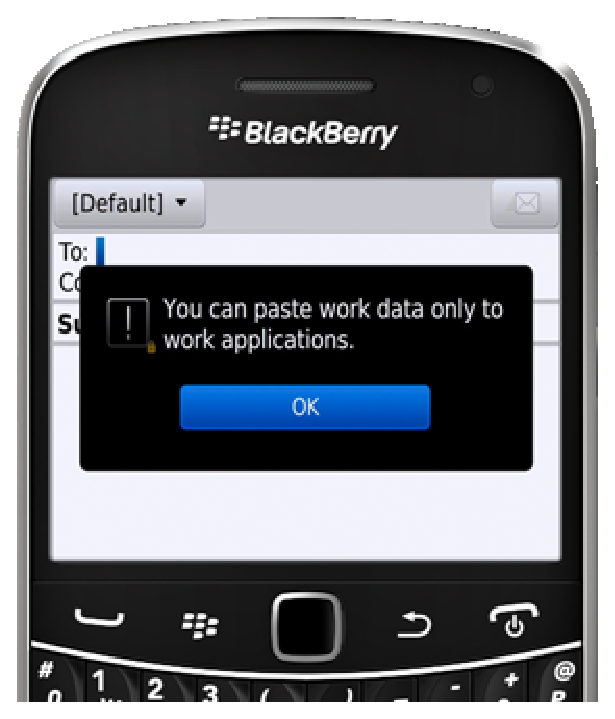
\includegraphics[scale=0.5]{img/Blackberry_balance.eps}
		\caption{Displayed message in new Blackberry 10 when attepmting to copy sensitive company data. Source: http://uk.blackberry.com/business/software/blackberry-balance.html.}
	\label{fig:blackberry_bal}
\end{figure}

On the other side, employees are able to access information and applications related to their personal lives, while staying connected to important work information when they need to perform. Finally, another known feature is also offered by Blackberry, so if the device gets lost or is stolen, or if the employee leaves the organization, there will be an option to wipe just work information which can be done remotely.


%----------------------------------------------------------------------------
%%%%%%%%%%%%%%%%%%%%%%%%%%%%%%%%   MUSES %%%%%%%%%%%%%%%%%%%%%%%%%%%%%%%%%%%%
%----------------------------------------------------------------------------


\section{Multiplatform Usable Endpoint Security System}
\label{sec:muses}

The MUSES system overview is presented in Figure \ref{fig:system_overview}. As it can be seen, in this system, the user interacts with the devices, own or corporate, through the MUSES graphical interface inside his or her own context (situation, connection, status). 

\begin{figure}[ht]
\centering
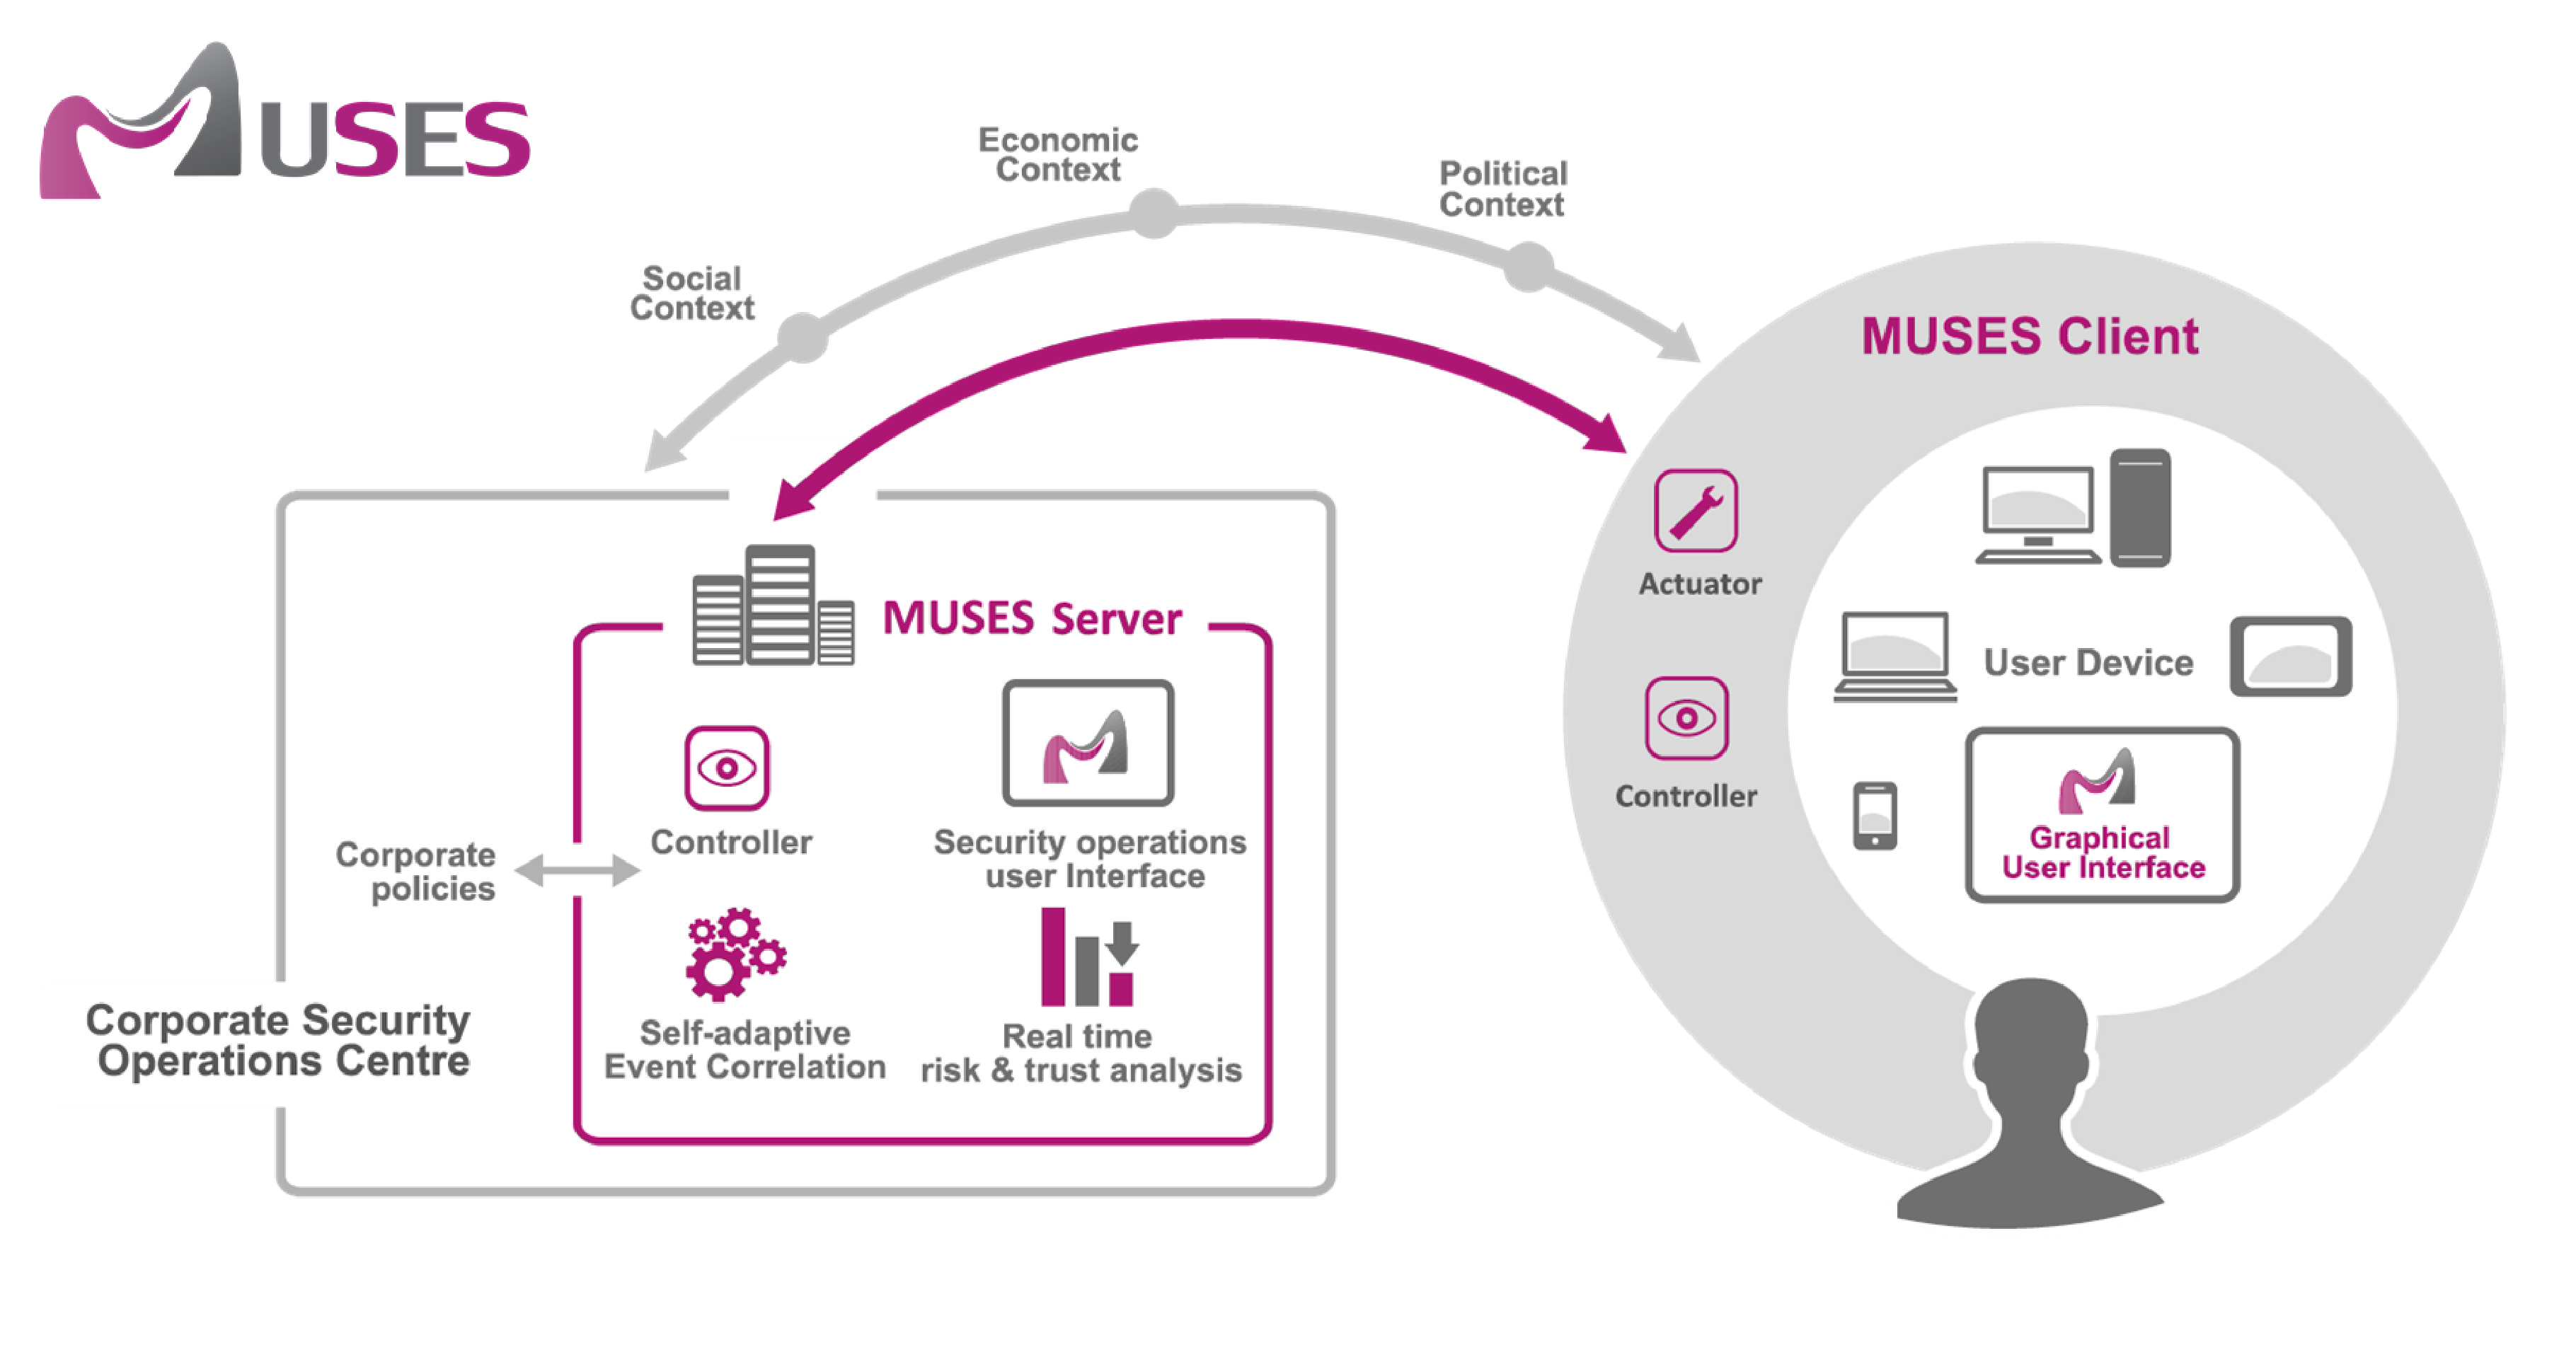
\includegraphics[scale=0.2]{img/system_overview2.eps}
\caption{MUSES system overview. (Design art by S2 Grupo.  http://www.s2grupo.es/.)\label{fig:system_overview}}
\end{figure}

As a summary, this application includes two modules: a \textit{controller} and an \textit{actuator}. The first one monitors the environment (context) and the user's behaviour, translating his/her actions into a sequence of events. These events, along with the patterns defining the user's conduct, are processed by the system in real-time by means of a Risk and Trust Analysis Engine (RT2AE) and an Event Correlation module. Then, a decision is taken in the corporate security operations centre (SOC) side, considering the RT2AE output and the set of security rules adapted to that specific user and context. The corresponding feedback is communicated to the user through the \textit{actuator}, which is also in charge of triggering the recommended actions to stop the user's or application's doings, in case it is required.

The designed MUSES architecture is shown in Figure \ref{fig:architecture}. It is a \textit{client/server} approach in which the \textit{client} program will be installed in every user's mobile or portable device, independently of the platform (operating system and type of device). The \textit{server} side would be installed in the corporate SOC. Both sides are connected through a secure channel (using HTTPS) over Internet. In that figure just the high-level components in each part are shown, along with the information flows labelled as 'Info XX'.

\begin{figure}[ht]
%\begin{center}
\hspace{-0.7in}
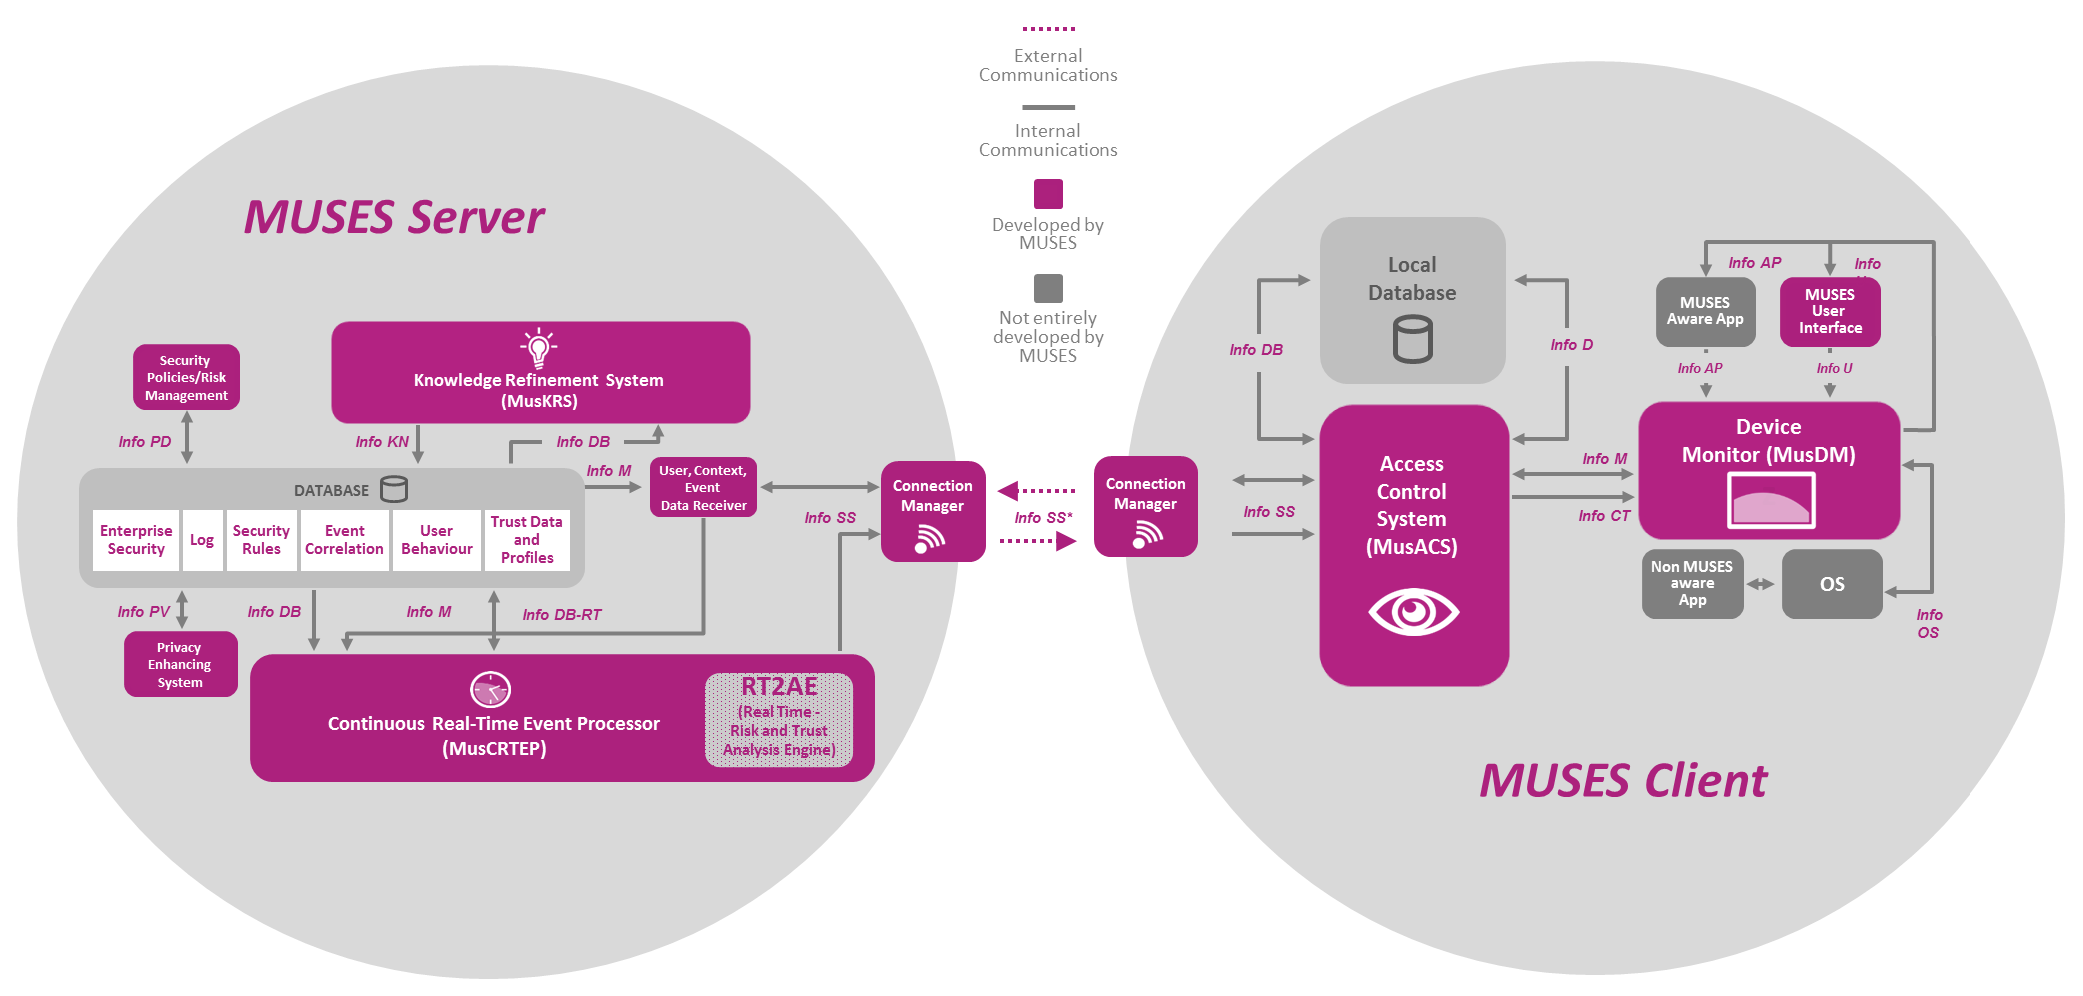
\includegraphics[scale=0.45]{img/architecture_modules.eps}
%\includegraphics[scale=0.45]{img/muses_architecture.eps}
\caption{Proposed architecture. (Design art by S2 Grupo. http://www.s2grupo.es/). \label{fig:architecture}}
%\end{center}
\end{figure}

The rationale for this approach is based on two main reasons: 1) there is need for a high computational power in order to perform the event correlation and self-adaptation processes, so a quite powerful machine should be used (server); 2) there are two clearly separated parts in the system, namely the users (client) and the enterprise (server).

The system considers two working modes for every device: online and offline. In the \textit{online} mode the device can connect with the MUSES server, so it can request the server to make a decision. On the other hand, in \textit{offline} mode the server cannot be reached by the device (there is not an available connection between them), so all the decisions should be made locally. Anyway, in this mode, the gathered information by the sensors in the device will be stored for later submission to the server side (when a connection is available), in order to be processed in the knowledge refinement process.

% ----------------------------------------------------------

\subsection{Client/Device architecture}

There are three main components in this side:
\begin{itemize}
 	 \item \textit{Local Database}: it is a local security-based storage, which includes the set of security rules to be applied locally (Device Policies), user authentication data, and a cache of gathered events and information. The latter will be useful when the device is in offline mode, so these data are stored to be later submitted to the server side. 
%It contains the so-called \textit{Decision Table}, a set of rules in which the antecedents are high-level events, and the consequents are the corresponding decisions/actions, namely `allow', `deny' or `request' (the decision must be made in the server side).
 	 \item \textit{Device Monitor (MusDM)}: module which gathers the events and information produced by the user. It also acts following the decisions made by the system, in order to allow or deny the controlled application (or the user) for doing something. It is composed by a monitoring and an actuator submodules.
 	 \item \textit{Access Control System (MusACS)}: module in charge of making the decisions considering the gathered data. These decisions can be made locally (if possible), or can be requested to the server (if there is no rule which matches with the occurred events). 

%The subcomponents are the \textit{Decision Maker}, which performs the decision process; the \textit{User, Context, Event Handler}, which processes the events and information to be used for making the decision or stored for further submission (depending on the mode and on the gathered data); and the \textit{Security Policy Receiver} that updates the set of decisions (or Device Policies) in the Decision Table with those received from the server side, after an update or decision process.
\end{itemize}

The rest of the components are: the \textit{MUSES User Interface (UI)}, the application through which the user interacts with the system; and the \textit{Connection Manager} which controls the communications between client and server sides. 
In addition, there are two types of applications considered in this system: on the one hand the \textit{MUSES Aware App}, which is an application adapted to MUSES, so the system can directly interact with it (monitoring and acting). This application must be implemented using the MUSES API (Application Program Interface)\footnote{The MUSES API will be defined in the project, so for every application desired to be MUSES Aware, it should be implemented using this.}. On the other hand the \textit{Non MUSES Aware App} is that which MUSES cannot directly interact with. Usually it will be accessed through the operating system (OS).

% ----------------------------------------------------------

\subsection{Server architecture}

As in the client, there are three main components:
\begin{itemize}
	 \item \textit{System Database}: it stores all the information that the system will manage, including authentication data, enterprise security policies, assets' values, user-related information (trust, context), events data, and, of course, security rules to apply (regarding the security policies).

	 \item \textit{Continuous Real-Time Event Processor (MusCRTEP)}: this component is the core of the MUSES system with respect to the decision making process. It includes an \textit{Event Processor}, the module in charge of performing the event correlation process \cite{EventProcessing_Luckham02,SurveyEventCorrelation_Tiffany02}, gathering the set of occurred events and doing a rule-based threat identification. The output of this module is taken by the \textit{RT2AE}, which also considering information such as trust data and profiles, assets' values, user reputation, or opportunity, performs a risk and trust analysis task \cite{RT2AE_SOTICS13}, and extracts the set of potential rules to consider in the analysed situation. Then, these rules are transformed into decisions (or Device Policies) and submitted to those devices to which they apply.

	 \item \textit{Knowledge Refinement System (MusKRS)}: this module is in charge of analysing the information stored in the system database, identifying relevant data, such as important patterns, key features, or security incidents. These are later processed for tuning up the existing set of rules or for inferring new ones. 

\end{itemize}

There are some other components, namely: the \textit{Security Policies/Risk Management} tool, that lets the company's chief security officer (CSO) to define and manage Security Policies and Rules in a friendly way. It also lets the management of risk-related information, useful for the RT2AE process, such as the assets' values. The \textit{Privacy Enhancing System} which is a module aimed to fit with the legal compliance of the system regarding the user's data anonymisation. The \textit{User, Context, Event Data Receiver} is devoted to receive data from the device side (events, user-related, etc) and to distribute them among the components (storing in the database, and requesting the Event Processor to start the correlation task). Finally, there is another \textit{Connection Manager} which controls the communication with the device side.

As previously stated, one of the main features of the presented system will be the self-adaptation (to the user and context) of the set of security rules. To this end, the MusKRS's task will be run asynchronously to the system working. This process is composed by two steps: first, a Data Mining procedure \cite{DataMining_Lee01} will be performed, considering the whole amount of historic information mainly regarding user's behaviour and context. Some methods such as Clustering \cite{Clustering_Jain99} (grouping data), Pattern Recognition \cite{PatternMining_Han07} (usual situations identification), or Feature Selection \cite{FeatureSelection_Guyon03} (main variables/values in the data) will be applied. The second step consists in a refinement and inference process, performed by means of Machine Learning \cite{MachineLearning_Bishop06} and Computational Intelligence techniques. Regarding the latter, some methods will be used, such as Evolutionary or Genetic Algorithms \cite{EAs_Back96,GAs_Goldberg89} for parameters/values optimisation; or Genetic Programming \cite{GP_Koza92} for the modification of security rules.

Thus the set of rules will be adapted to every user in the system, updating some of the existing and creating new ones (always respecting the corporate security policies).
Moreover, some predictive models will be also obtained applying other soft computing techniques, so the user's potentially dangerous behaviour will be anticipated.


%
%
%
%The system architecture can be seen in Figure \ref{fig:architecture}. It is a client-server approach in which the \textit{client} program will be installed in every user's device independently of the platform (operative system and type of device). This client contains a \textit{Device Monitor} module, which gathers the performed sequence of events and user context information and transforms them into information manageable by the rest of components in the system. It also includes an \textit{Actuator submodule}, which will conduct the actions over the
%
%\textit{controller submodule} in charge of take some light decisions considering the server response to the current situation (it will also take the control in case the device cannot connect with the server). The device controller will trigger the \textit{actuator} if necessary. This module will provide the user with some feedback, and will interact with the applications being monitorized if recommended or required.
%
%The \textit{server} side would be installed in the corporate SOC. This application contains, in addition to an user interface to manage it, the main modules in the security-aimed decision process: the \textit{RT2AE} and the \textit{Event Correlator}. These components are connected between them and also with the main \textit{Controller}, that will connect with the device side sending the selected set of security rules that better fit with the current situation, along with the actions to be performed according to them.
%
%
%One of the main features of the presented system is the self-adaptation (to the user and context) of the set of rules. To this aim, asynchronously to the system working, there will be run a process which will consider the whole amount of historic information regarding user's behaviour and context, and refine it by means of computational intelligence and machine learning techniques. Thus the set of security rules will be adapted to the every user in the system, updating some of the existent rules and creating new ones (always respecting the corporate security policies).
%Moreover, some predictive models will be also obtained applying other soft computing techniques, so the user's potentially dangerous behaviour will be anticipated.


%----------------------------------------------------------------------------
%%%%%%%%%%%%%%%%%%%%%%%%%%%%%%%   COMPARISON  %%%%%%%%%%%%%%%%%%%%%%%%%%%%%%%
%----------------------------------------------------------------------------

\section{MUSES Advantages Against other Solutions. Beyond the State of the Art}
\label{sec:comparison}


MUSES is mainly a free, open-source, platform independent solution, so these set of features make it a very good option in a first comparison against the proprietary, close and system-specific tools presented in Section \ref{sec:toolsreview}. Moreover most of the existent tools take into account only smartphones and tablets, but MUSES also covers laptops and company PCs too. Moreover the companies which desires work with those systems need specific operative system and server (such as Windows Server, for instance). 
Being even more strict in some cases, as in Samsung Knox, in which companies must work with a specific (though they can choose from a list) MDM service for being able of deploy Knox in their environments. 


Another comparison concerns that the existing products are mostly policy-based, but MUSES makes its decisions not only considering policies, but also based on the terminals/users context (location, connected networks and so on), to really understand the real danger of a specific action.
Also related to this, a very big plus of the MUSES system is its new feature of self-adaptivity. Thus, MUSES is able to adapt to changes, either regarding corporate security policies, newly discovered vulnerabilities or threats, different environments of use or user profiles. 

Moreover, MUSES has the feature of having two connection modes, depending on the client being able to connect with the server or not, which favours a real-time decision making process.

Though these are clearly advantages of MUSES over the aforementioned products, they also establish a progress beyond the state of the art. Other issues that MUSES aims to progress on are related to risk and trust data analysis, human-computer interaction (or HCI), device monitoring, and legal compliance. First, as mentioned previously, it will implement a self-adaptive event correlation, including a novel hybrid technique of rule refinement and rule adjustment extracting relevant information from processing huge amounts of data. Then, the project defines a new approach to risk management taking into account threats (with their costs) as well as the innovative concept of opportunity, i.e. the following beneficial outcome from a situation on which, for instance, a user is able to work while waiting at the airport if risk is low enough. About HCI and usability of mobile devices, this will set up a significant advance in the state of the art because of the novelty of the BYOD philosophy, and trying to look for individual differences among the users in susceptibility to persuasive strategies for secure behaviour. Regarding device monitoring, MUSES will also take into account the so-called context observation, by which private or professional scenarios will be detected, or predicted, based on advanced machine learning techniques. Finally, the project is concerned about legal compliance in regards of Information Security Policies, so that it will contribute to the proposal for the EU Data Protection: legal binding force and legal certainty of company policies, and end-user responsibility.


%----------------------------------------------------------------------------
%%%%%%%%%%%%%%%%%%%%%%%%%%%%%%%   CONCLUSIONS  %%%%%%%%%%%%%%%%%%%%%%%%%%%%%%%
%----------------------------------------------------------------------------

\section{Conclusions}
\label{sec:conclusions}

In this work, there are presented several tools that prove how information security in the enterprise is adapting to this emergent philosophy of BYOD. For each one, the main features and working environments were detailed. Also it was shown, by the introduction to MUSES project, how the European Community is specially aware about that and is developing a free solution for managing employees privacy, and securing companies' assets in this changing environment. 

MUSES architecture has been described and its main advantages with respect to the other solutions has been presented, also remarking its advances beyond the state of the art that define these tools.

The paper has been written through a vast literature review; the tools were not possible to be tested because, in the first place, all of them but MUSES are neither free nor open source and, secondly, some of them has just been released, such as the Samsung Knox (release delayed from April/May to the end of 2013) or even MUSES, which first prototype is about to be released in some weeks.
Anyway, this work can be useful as a survey of the existent tools, regarding some important topics in security nowadays, such as the security policies use, the end-to-end solutions, the mixture between data security and privacy, or the risk analysis, to cite a few.

%%%%%%%%%%%%%%%%%%%%%%%%%%%%%  ACKNOWLEDGEMENTS %%%%%%%%%%%%%%%%%%%%%%%%%%%%%%%%

\section{Acknowledgements}
This work has been supported by MUSES FP7 project, and in part by the P08-TIC-03903 project awarded by the Andalusian Regional Government, the FPU Grant 2009-2942, and the TIN2011-28627-C04-02 project, awarded by the Spanish Ministry of Science and Innovation.

\bibliographystyle{elsarticle-num}

% Antonio - Poner la bibliograf�a en fichero .bib

\begin{thebibliography}{00}

%\bibitem{ids13}
%Sommestad T., Hunstad A.. \emph{Intrusion detection and the role of the system administrator.}, from Swedish Defence Research Agency (FOI), Link�ping, Sweden, 2013.

%\bibitem{m2m12}
%NTT DOCOMO, \emph{DOCOMO to Launch Global M2M Platform}, in M2M Magazine, December 2012.
%http://www.machinetomachinemagazine.com/2012/12/05/docomo-to-launch-global-m2m-platform/.

%\bibitem{suites12}
%The Radicati Group Inc., report \emph{Microsoft Office 365 - Analysis and Forecast, 2012-2016}. June 2012. 

\bibitem{Adams_Users05}
Adams, A. and Sasse, A.:
\newblock {\em Users are not the enemy}.
\newblock Security and Usability: Designing Systems That People Can Use.
  O\'Reilly Associations, 2005.

\bibitem{SecPolComp12}
Al-Omari, A., El-Gayar, O., Deokar, A., and Walters, J.: \emph{Security Policy Compliance: User Acceptance Perspective}. 45th Hawaii International
Conference on System Sciences (pp. 3317-3326). IEEE, 2012.

\bibitem{BYOD13}
Bacik, S.: \emph{Security Implications of Bring Your Own Device, IT Consumerization, and Managing User Choices}, in Information Security Management Handbook, Sixth Edition, Volume 7, pp. 133-142, 2013.

\bibitem{EAs_Back96}
Back, T.:
\newblock {\em Evolutionary algorithms in theory and practice}.
\newblock Oxford University Press, 1996.

\bibitem{MachineLearning_Bishop06}
Bishop, C.:
\newblock {\em Pattern recognition and Machine Learning}.
\newblock Springer, 2006.

\bibitem{Blackberry_tool}
Blackberry.
\newblock Blackberry balance.
\newblock http://es.blackberry.com/business/software/blackberry-balance.html.

\bibitem{SecPolComp10}
Bulgurcu, B., Cavusoglu, H., and Benbasat, I.: \emph{Information security policy compliance: an empirical study of rationality-based beliefs and information security awareness}. MIS Quarterly, 34(3), 523-548. 2010.

\bibitem{SecPol09}
Cresson Wood, C. and Lineman, D.: \emph{Information Security Policies Made Easy Version 11}. Information Shield, Inc. 2009.

\bibitem{Good_tool}
Good's Technology.
\newblock BYOD Solution.
\newblock
  http://www1.good.com/secure-mobility-solution/bring-your-own-device.html.

\bibitem{GAs_Goldberg89}
Goldberg, D.E.:
\newblock {\em Genetic Algorithms in search, optimization and machine
  learning}.
\newblock Addison Wesley, 1989.

\bibitem{FeatureSelection_Guyon03}
Guyon, I.,  and Elisseeff, A.:
\newblock An introduction to variable and feature selection.
\newblock {\em J. Mach. Learn. Res.}, 3:1157--1182, 2003.

\bibitem{PatternMining_Han07}
Han, J., Cheng, H., Xin, D., and Yan, X.:
\newblock Frequent pattern mining: Current status and future directions.
\newblock {\em Data Min. Knowl. Discov.}, 15(1):55--86, 2007.

\bibitem{SecPolPenalty09}
Herath, T., and Rao, H.R.: \emph{Protection motivation and deterrence: a framework for security policy compliance in organisations}. European Journal of Information Systems, vol. 18, pp. 106-125, 2009.
	
\bibitem{IBM_tool}
IBM.
\newblock Hosted mobile device security management.
\newblock
http://www-935.ibm.com/services/us/en/it-services/managed-security-services-cloud-computing-hosted-mobile-device-security-management.html.

\bibitem{Clustering_Jain99}
Jain, A.K., Murty, M.N., and Flynn, P.~J.:
\newblock Data clustering: A review.
\newblock {\em ACM Comput. Surv.}, 31(3):264--323, Sept. 1999.

\bibitem{GP_Koza92}
Koza, J.~R.:
\newblock {\em Genetic Programming: On the programming of computers by means of
  natural selection}.
\newblock MIT Press, Cambridge, MA, 1992.
	
\bibitem{ibm11}
Kao, I-L.: \emph{IBM Security Services. Securing mobile devices in the business environment}, IBM, 2011.

\bibitem{DataMining_Lee01}
Lee, S.J. and Siau, K.:
\newblock A review of data mining techniques.
\newblock {\em Industrial Management \& Data Systems}, 101(1):41--46, 2001.

\bibitem{MIT05}
Lippmann, R.P., Ingols, K.W., Scott, C., Piwowarski, K., Kratkiewicz, K.J., Artz, M., and Cunningham, R.K.: \emph{Evaluating and Strengthening Enterprise
Network Security Using Attack Graphs}. Project Report IA-2. Lincoln Laboratory, Massachusetts Institute of Technology, October 2005.

\bibitem{EventProcessing_Luckham02}
Luckham, D..
\newblock {\em The Power of Events: An Introduction to Complex Event Processing
  in Distributed Enterprise Systems}.
\newblock Addison-Wesley, MA, USA, 2002.

\bibitem{Opp_Security11}
Oppliger, R.:
\newblock Security and privacy in an online world.
\newblock {\em IEEE Computer}, 44(9):21--22, September 2011.

\bibitem{android11}
Orthacker, C., Teufl, P., Kraxberger, S., Lackner, G., Gissing, M., Marsalek, A., Leibetseder, J., and Prevenhueber, O.: \emph{Android Security Permissions - Can We Trust Them?}. MobiSec Session on Smartphone Security, Aalborg 2011.

\bibitem{SecPolComp09}
Shaw, R.S., Chen, C.C., Harris, A.L., and Huang, H.-J.: \emph{The impact of information richness on information security 
awareness training effectiveness}. Computers \& Education, vol. 52, pp. 92-100, 2009.

\bibitem{Samsung_tool}
Samsung KNOX.
\newblock
  https://www.samsungknox.com.

\bibitem{Schu_SecPatterns05}
Schumacher, M., Fernandez-Buglioni, E., Hybertson, D., Buschmann, F., and
  Sommerlad, P.:
\newblock {\em Security Patterns: Integrating Security and Systems
  Engineering}.
\newblock John Wiley \& sons, 2005.

\bibitem{RT2AE_SOTICS13}
Seigneur, J.-M., K�lndorfer, P., Busch, M., and Hochleitner, C.:
\newblock A survey of trust and risk metrics for a byod mobile working world.
\newblock In {\em Third International Conference on Social Eco-Informatics
  (SOTICS 2013)}, page To Appear. Curran Associates Inc., November 2013.

\bibitem{SecPolComp07}
Siponen, M., Pahnila, S., and Mahmood, A.: \emph{Employees' adherence to information security policies: an empirical study}. In IFIP International Federation for Information Processing, Volume 232, New Approaches for Security, Privacy and Trust in Complex Environments pp. 133-144, 2007.
	
\bibitem{Sophos_tool}
Sophos.
\newblock Mobile control.
\newblock http://www.sophos.com/en-us/products/mobile-control.aspx.

\bibitem{SurveyEventCorrelation_Tiffany02}
Tiffany, M.:
\newblock A survey of event correlation techniques and related topics.
\newblock Research paper, Georgia Institute of Technology, 2002.


\end{thebibliography}

\end{document}
